\ifx\pdfminorversion\undefined\else\pdfminorversion=4\fi
\documentclass[aspectratio=169,t]{beamer}
%\documentclass[aspectratio=169,t,handout]{beamer}

% English version FAU Logo
\usepackage[english]{babel}
% German version FAU Logo
%\usepackage[ngerman]{babel}

\usepackage[utf8]{inputenc}
\usepackage[T1]{fontenc}
\usepackage{amsmath,amssymb}
\usepackage{graphicx}
\usepackage{listings}
\usepackage{url}
\usepackage{hyperref}
\usepackage{fontawesome}
\usepackage{tikz}
\usepackage{tikz-cd}

\tikzset{
    vertex/.style = {
        circle,
        fill            = black,
        outer sep = 2pt,
        inner sep = 1pt,
    }
}
\usetikzlibrary{matrix}
\usetikzlibrary{arrows,decorations.pathmorphing,backgrounds,fit,positioning,shapes.symbols,chains,intersections}
% Options:
%  - inst:      Institute
%                 med:      MedFak FAU theme
%                 nat:      NatFak FAU theme
%                 phil:     PhilFak FAU theme
%                 rw:       RWFak FAU theme
%                 rw-jura:  RWFak FB Jura FAU theme
%                 rw-wiso:  RWFak FB WISO FAU theme
%                 tf:       TechFak FAU theme
%  - image:     Cover image on title page
%  - plain:     Plain title page
%  - longtitle: Title page layout for long title
\usetheme[%
  image,%
  longtitle,%
  tf
]{fau}

% Enable semi-transparent animation preview
\setbeamercovered{transparent}


\lstset{%
  language=Python,
  tabsize=2,
  basicstyle=\tt,
  keywordstyle=\color{blue},
  commentstyle=\color{green!50!black},
  stringstyle=\color{red},
  numbers=left,
  numbersep=0.5em,
  xleftmargin=1em,
  numberstyle=\tt
}


% Title, authors, and date
\title[KDD]{Chapter I: Introduction}
\subtitle{Knowledge Discovery in Databases}
\author[L.~Melodia]{Luciano Melodia M.A.}
% English version
\institute[Department]{Evolutionary Data Management, Friedrich-Alexander University Erlangen-Nürnberg}
% German version
%\institute[Lehrstuhl]{Lehrstuhl, Friedrich-Alexander-Universit\"at Erlangen-N\"urnberg}
\date{Summer semester 2021}
% Set additional logo (overwrites FAU seal)
%\logo{\includegraphics[width=.15\textwidth]{themefau/art/xxx/xxx.pdf}}


\begin{document}
  % Title
  \maketitle

  { 
    \setbeamertemplate{footline}{}
    \begin{frame}{Chapter I: Introduction}
    This is our agenda for this lecture:
        \begin{itemize}
            \item \textbf{Why data mining?}
            \item What is data mining?
            \item A multi-dimensional view of data mining.
            \item What kind of data can be mined?
            \item What kinds of patterns can be mined?
            \item What technologies are used?
            \item What kinds of applications are targeted?
            \item Major issues in data mining.
            \item A brief history of data mining.
            \item Summary.
        \end{itemize}
    \end{frame}
  }

  { 
    \setbeamertemplate{footline}{}
    \begin{frame}{Why data mining?}
    \textbf{The explosive growth of data: from terabytes to petabytes and more.}\\
        \begin{itemize}
            \item Data collection and availability:
                \begin{itemize}
                    \item Automated data collection tools.
                    \item Database systems.
                    \item World wide web.
                    \item Computerized society.
                    \item Digitization.
                \end{itemize}
            \item Major sources of abundant data:
                \begin{itemize}
                    \item Business: web, e-commerce, transactions, stocks \ldots
                    \item Science: remote sensing, bioinformatics, scientific simulation \ldots
                    \item Society: news, digital cameras, social media \ldots
                \end{itemize}
            \item The era of \textbf{big data} (as inflationary used buzzword).
        \end{itemize}
    \textbf{We are drowning in data, but starving for knowledge.} \textbf{Necessity is the mother of invention.}\\
    For data mining it is the automated analysis of massive data sets.
    \end{frame}
  }

  { 
    \setbeamertemplate{footline}{}
    \begin{frame}{Evolution of sciences I}
        \begin{itemize}
            \item Before $1600$, era of \textbf{empirical science}.
            \item $1600-1950$s, rise of \textbf{theoretical science}.
                  \begin{itemize}
                      \item Each discipline has grown a theoretical component.
                      \item Theoretical models often motivate experiments and generalize our understanding.
                  \end{itemize}
            \item $1950-1990$s, rise of \textbf{computational science}.
                  \begin{itemize}
                      \item Over the last $50$ years most disciplines have grown a third, computational branch.
                      \begin{itemize}
                          \item E.g. empirical, theoretical and computational ecology.
                          \item E.g. physics, linguistics or biology.
                      \end{itemize}
                  \end{itemize}
            \item Computational science traditionally meant simulation.
            \item It grew out of our inability to describe reality by closed-form mathematical models.
        \end{itemize}
    \end{frame}
  }

  { 
    \setbeamertemplate{footline}{}
    \begin{frame}{Evolution of sciences II}
        \begin{itemize}
            \item $1990-$now, rise of \textbf{data science}.
                  \begin{itemize}
                      \item The flood of data from new instruments and modern simulations.
                      \item The ability to economically store and manage petabytes of data.
                      \item The internet makes all these archives world wide accessible.
                      \item Scientific \emph{information management}, \\
                            acquisition,\\
                            organization, \\
                            query and \\
                            visualization scale almost linearly with amount of data.
                      \item \textbf{Data mining} is a major new challenge!
                  \end{itemize}
          \item For further reading:\\
                \small{Jim Gray and Alex Szaly: \emph{The World Wide Telescope: An Archetype for Online Science}, \\ Communications of the ACM 45(11): 50-54, 2002.}
        \end{itemize}
    \end{frame}
  }

  { 
    \setbeamertemplate{footline}{}
    \begin{frame}{Evolution of sciences III}
        \begin{itemize}
            \item $1960$s: Data collection, \\
                  \hspace{1cm} database creation, \\
                  \hspace{1cm} integrated management systems (IMS) and \\
                  \hspace{1cm} network database management systems (DBMS).
            \item $1970$s: Relational data model, relational DBMS implementation (RDBMS).
            \item $1980$s: RDBMS products,\\
                  \hspace{1cm} database creation, \\
                  \hspace{1cm} advanced data models (extended relational, object oriented, deductive etc.),\\
                  \hspace{1cm} application-oriented DBMS (spatial, scientific, engineering etc.).
            \item $1990$s: Data mining,\\
                  \hspace{1cm} data warehousing, \\
                  \hspace{1cm} multimedia databases,\\
                  \hspace{1cm} web databases.
            \item $2000$s: Stream data management and mining,\\
                  \hspace{1cm} data mining and applications, \\
                  \hspace{1cm} web technology (XML, data integration) and global information systems.
        \end{itemize}
    \end{frame}
  }

  { 
    \setbeamertemplate{footline}{}
    \begin{frame}{Chapter I: What is data mining?}
        \begin{itemize}
            \item Why data mining?
            \item \textbf{What is data mining?}
            \item A multi-dimensional view of data mining.
            \item What kind of data can be mined?
            \item What kinds of patterns can be mined?
            \item What technologies are used?
            \item What kinds of applications are targeted?
            \item Major issues in data mining.
            \item A brief history of data mining.
            \item Summary.
        \end{itemize}
    \end{frame}
  }

  { 
    \setbeamertemplate{footline}{}
    \begin{frame}{What is data mining?}
    \textbf{Data mining or knowledge discovery from data}:
        \begin{itemize}
            \item Extraction of interesting (\textbf{non-trivial, implicit, previously unknown \\
                  and potentially useful}) patterns from huge amounts of data.
            \item Is \textbf{data mining} a misnomer?
        \end{itemize}
    Alternative names:
        \begin{itemize}
            \item Knowledge discovery/mining in databases (KDD).
            \item Knowledge extraction.
            \item Data/pattern analysis.
            \item Data archeology.
            \item Data dredging.
            \item Information harvesting.
            \item Business intelligence.
        \end{itemize}
    Watch out: Is everything \textbf{data mining}?
        \begin{itemize}
            \item Simple search and query processing is considered not to be.
            \item Neither are deductive expert systems.
        \end{itemize}
    \end{frame}
  }


  { 
    \setbeamertemplate{footline}{}
    \begin{frame}{Knowledge discovery pipeline}
    \begin{itemize}
        \item This is a typical view from a typical database-systems and data-warehousing community.
        \item Data mining plays an essential role in the knowledge-discovery process.
    \end{itemize}
 
    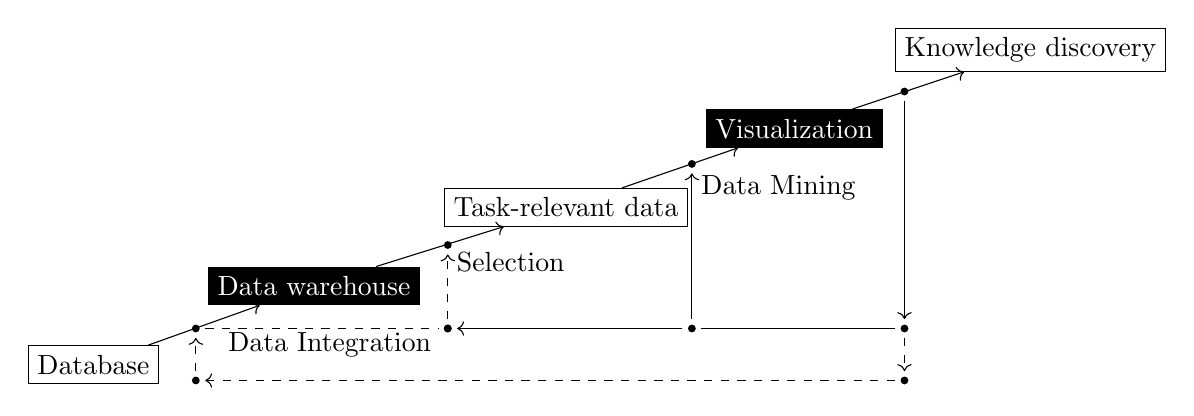
\begin{tikzpicture}
      % Dialectics
      \node[draw] (Database) at (0,0) {Database};
      \node[draw,fill=black,text=white] (Data warehouse) at (2.8,1) {Data warehouse};
      \node[draw] (Task-relevant data) at (6,2) {Task-relevant data};
      \node[draw,fill=black,text=white] (Data mining) at (8.9,3) {Visualization};
      \node[draw] (Knowledge discovery) at (11.9,4) {Knowledge discovery};

      \node (Data Integration) at (3,0.25) {Data Integration};
      \node (Selection) at (5.3,1.3) {Selection};
      \node (Data Mining) at (8.7,2.25) {Data Mining};

      \draw node[vertex] (Joint1) at (1.3,0.46) {};
      \draw node[vertex] (Joint2) at (4.5,1.52) {};

      \draw node[vertex] (Joint3) at (4.5,0.46) {};
      \draw node[vertex] (Joint7) at (4.5,0.46) {};
      \draw node[vertex] (Joint8) at (7.6,0.46) {};
      \draw node[vertex] (Joint9) at (10.3,0.46) {};
      \draw node[vertex] (Joint10) at (10.3,-0.2) {};
      \draw node[vertex] (Joint11) at (1.3,-0.2) {};

      \draw node[vertex] (Joint5) at (7.6,2.55) {};
      \draw node[vertex] (Joint6) at (10.3,3.47) {};


      \draw[->,draw=black] (Database) to (Data warehouse);
      \draw[->,draw=black] (Data warehouse) to (Task-relevant data);
      \draw[->,draw=black] (Task-relevant data) to (Data mining);
      \draw[->,draw=black] (Data mining) to (Knowledge discovery);
      \draw[-,draw=black, dashed] (Joint1) to (Joint3);
      \draw[->,draw=black, dashed] (Joint3) to (Joint2);
      \draw[->,draw=black] (Joint6) to (Joint9);
      \draw[-,draw=black] (Joint9) to (Joint8);
      \draw[->,draw=black] (Joint8) to (Joint7);
      \draw[->,draw=black] (Joint8) to (Joint5);
      \draw[->,draw=black,dashed] (Joint10) to (Joint11);
      \draw[->,draw=black,dashed] (Joint9) to (Joint10);
      \draw[->,draw=black,dashed] (Joint11) to (Joint1);
      \end{tikzpicture}
    \end{frame}
  }

   { 
    \setbeamertemplate{footline}{}
    \begin{frame}{Example: a web-mining framework}
    \textbf{Web mining usually involves:}
    \begin{itemize}
        \item Data cleaning.
        \item Data integration from multiple sources.
        \item Warehousing the data.
        \item Data-cube construction.
        \item Data selection for data mining.
        \item Data mining.
        \item Presentation of the mining results.
        \item Patterns and knowledge to be used or stored in a knowledge base.
    \end{itemize}
    \end{frame}
  }

  { 
    \setbeamertemplate{footline}{}
    \begin{frame}{Data mining in business}
    \centering
    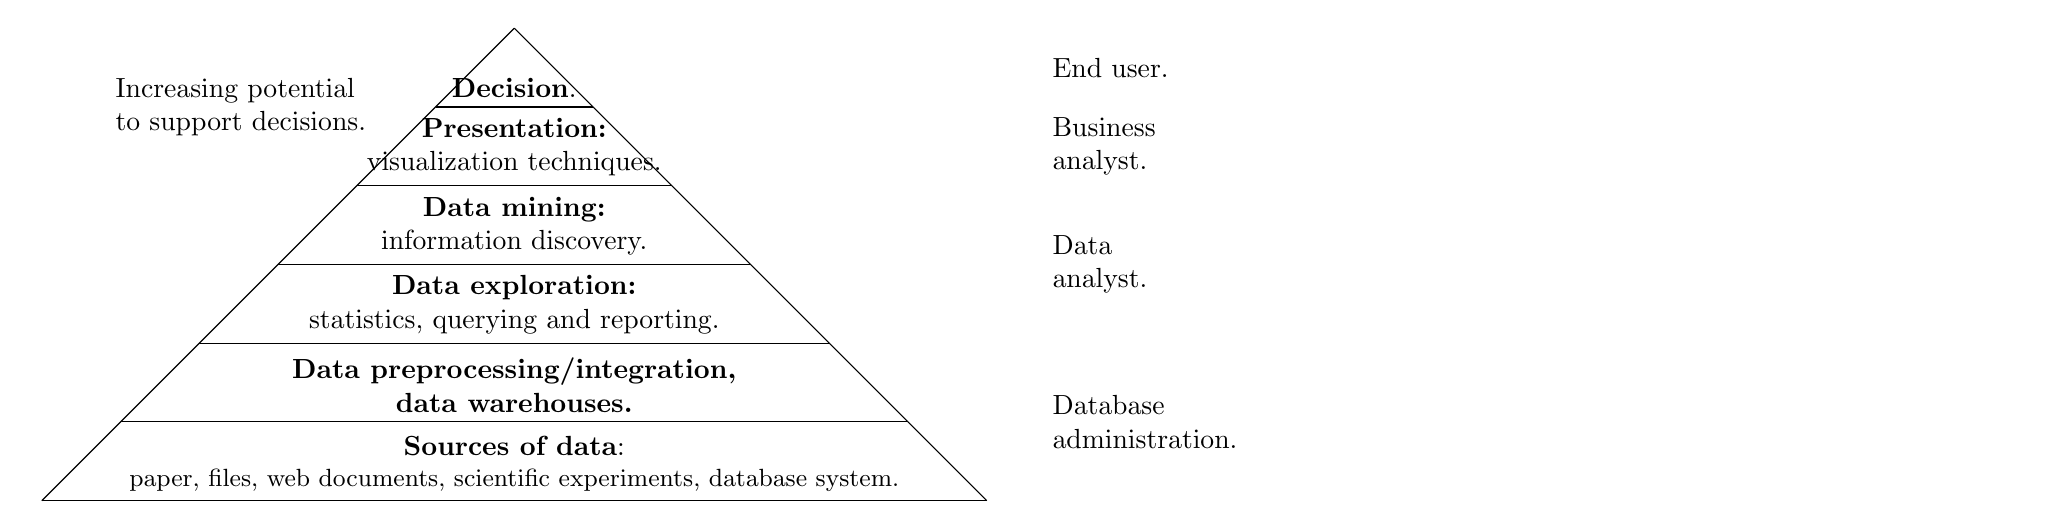
\begin{tikzpicture}
    \coordinate (A) at (-6,0) {};
    \coordinate (B) at ( 6,0) {};
    \coordinate (C) at (0,6) {};
    \draw[name path=AC] (A) -- (C);
    \draw[name path=BC] (B) -- (C);

    \node (Data Integration) at (1,5) {\parbox{\linewidth}{Increasing potential \\ to support decisions.}};
    \node (Data Integration) at (12.9,1) {\parbox{\linewidth}{Database \\ administration.}};
    \node (Data Integration) at (12.9,3) {\parbox{\linewidth}{Data \\ analyst.}};
    \node (Data Integration) at (12.9,4.5) {\parbox{\linewidth}{Business \\ analyst.}};
    \node (Data Integration) at (12.9,5.5) {\parbox{\linewidth}{End user.}};

    \foreach \y/\A in {0/{
        \parbox{\linewidth}{\centering \textbf{Sources of data}: \\ \small{paper, files, web documents, scientific experiments, database system.}}},
        1/\parbox{\linewidth}{\centering \textbf{Data preprocessing/integration,\\ data warehouses.}},
        2/\parbox{\linewidth}{\centering \textbf{Data exploration:} \\ statistics, querying and reporting.},
        3/\parbox{\linewidth}{\centering \textbf{Data mining:} \\ information discovery.},
        4/\parbox{\linewidth}{\centering \textbf{Presentation:} \\ visualization techniques.},
        5/\parbox{\linewidth}{\centering \textbf{Decision}.}} {
        \path[name path=horiz] (A|-0,\y) -- (B|-0,\y);
        \draw[name intersections={of=AC and horiz,by=P},
              name intersections={of=BC and horiz,by=Q}] (P) -- (Q)
            node[midway,above] {\A};
    }
    \end{tikzpicture}
    \end{frame}
  }

  { 
    \setbeamertemplate{footline}{}
    \begin{frame}{Example: mining vs. data exploration}
    \begin{itemize}
        \item Business intelligence view:
        \begin{itemize}
            \item Warehouse, data cube or reporting.
            \item But not much mining.
        \end{itemize}
        \item Business objects vs. data mining tools.
        \item Supply chain example: tools.
        \item Data presentation.
        \item Exploration.
    \end{itemize}
    \end{frame}
  }

  { 
    \setbeamertemplate{footline}{}
    \begin{frame}{KDD pipeline: a typical view from machine learning and statistics}
    \begin{itemize}
        \item This is a view from typical machine-learning and statistics communities.
    \end{itemize}
    \vspace{0.5cm}
    \centering
    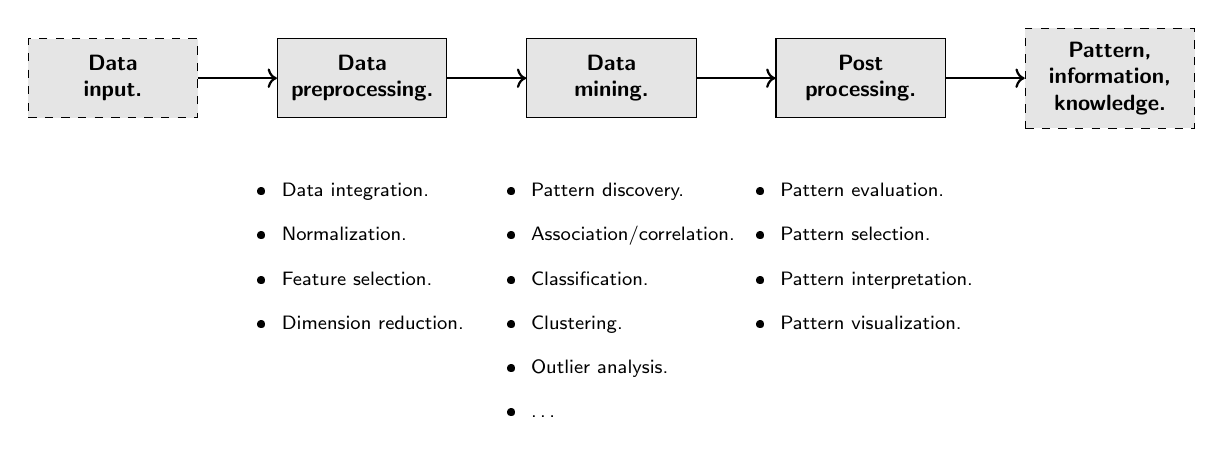
\begin{tikzpicture}
    [node distance = 1cm, auto,font=\footnotesize,
    % STYLES
    every node/.style={node distance=1cm},
    % The comment style is used to describe the characteristics of each force
    comment/.style={rectangle, inner sep= 5pt, text width=3.8cm, node distance=0.5cm, font=\scriptsize\sffamily},
    % The force style is used to draw the forces' name
    force/.style={rectangle, draw, fill=black!10, inner sep=5pt, text width=1.8cm, text badly centered, minimum height=1cm, font=\bfseries\footnotesize\sffamily}] 

    % Draw forces
    \node [force, dashed] (a) {\parbox{\linewidth}{\centering Data \\ input.}};
    \node [force, right=1cm of a] (b) {\parbox{\linewidth}{\centering Data \\ preprocessing.}};
    \node [force, right=1cm of b] (c) {\parbox{\linewidth}{\centering Data \\ mining.}};
    \node [force, right=1cm of c] (d) {\parbox{\linewidth}{\centering Post \\ processing.}};
    \node [force, dashed, right=1cm of d] (e) {\parbox{\linewidth}{\centering Pattern, \\ information, \\ knowledge.}};

    %%%%%%%%%%%%%%%
    % Change data from here

    % SUPPLIERS
    \node [comment, below=0.25cm of b] {
    \begin{itemize}
        \item Data integration.
        \item Normalization.
        \item Feature selection.
        \item Dimension reduction.
    \end{itemize}
    };

    % USERS
    \node [comment, below=0.25 of c] {
    \begin{itemize}
        \item Pattern discovery.
        \item Association/correlation.
        \item Classification.
        \item Clustering.
        \item Outlier analysis.
        \item \ldots
    \end{itemize}
    };

    % PUBLIC POLICIES
    \node [comment, below=0.25 of d] {
      \begin{itemize}
        \item Pattern evaluation.
        \item Pattern selection.
        \item Pattern interpretation.
        \item Pattern visualization.
    \end{itemize}
    };

    \path[->,thick] 
    (a) edge (b)
    (b) edge (c)
    (c) edge (d)
    (d) edge (e);

    \end{tikzpicture} 
    \end{frame}
  }

  { 
    \setbeamertemplate{footline}{}
    \begin{frame}{Example: medical data mining}
    \begin{itemize}
        \item \textbf{Health care and medical data mining}:
        \begin{itemize}
            \item Often adopted such a view in statistics and machine learning.
        \end{itemize}
        \item \textbf{Preprocessing of data}:
        \begin{itemize}
            \item Includes feature extraction and dimension reduction.
        \end{itemize}
        \item \textbf{Classification and/or clustering processes.}
        \item \textbf{Post processing for presentation}.
    \end{itemize}
    \end{frame}
  }

 { 
    \setbeamertemplate{footline}{}
    \begin{frame}{CRISP-DM}
    \begin{itemize}
        \item \textbf{CRoss-Industry Standard Process for Data Mining}:
    \end{itemize}
      \vspace{0.5cm}
    \centering
    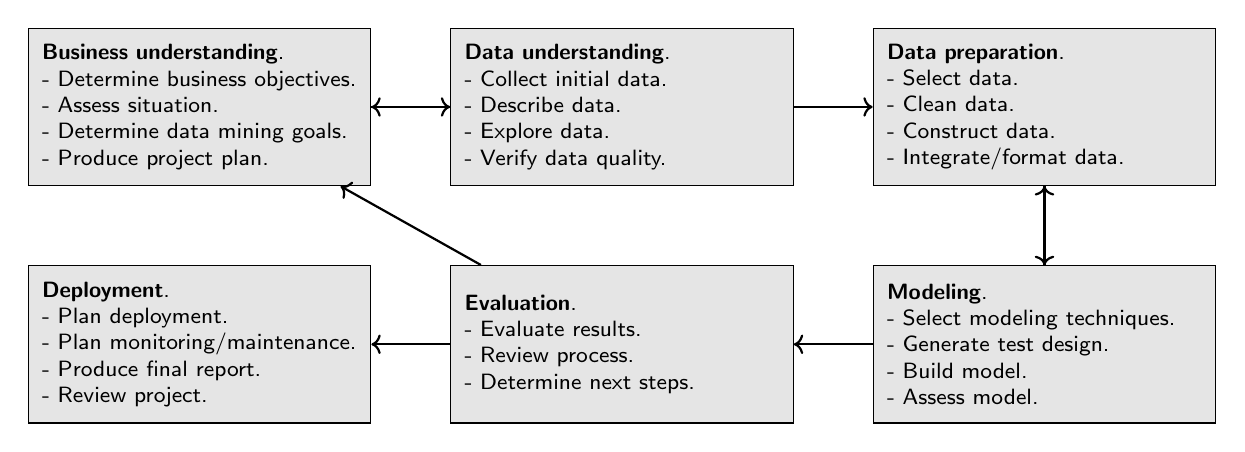
\begin{tikzpicture}
    [node distance = 2cm, auto,font=\footnotesize,
    % STYLES
    every node/.style={node distance=2cm},
    % The comment style is used to describe the characteristics of each force
    comment/.style={rectangle, inner sep= 5pt, text width=5cm, node distance=0.5cm, font=\scriptsize\sffamily},
    % The force style is used to draw the forces' name
    force/.style={rectangle, draw, fill=black!10, inner sep=5pt, text width=4cm, minimum height=2cm, font=\footnotesize\sffamily}] 

    % Draw forces
    \node [force] (a) {
    \parbox{\linewidth}{
    \textbf{Business understanding}.\\
    - Determine business objectives.\\
    - Assess situation.\\
    - Determine data mining goals.\\
    - Produce project plan.
    }
    };
    \node [force, right=1cm of a] (b) {
    \parbox{\linewidth}{
    \textbf{Data understanding}.\\
    - Collect initial data.\\
    - Describe data.\\
    - Explore data.\\
    - Verify data quality.
    }
    };
    \node [force, right=1cm of b] (c) {
    \parbox{\linewidth}{
    \textbf{Data preparation}.\\
    - Select data.\\
    - Clean data.\\
    - Construct data.\\
    - Integrate/format data.
    }
    };
    \node [force, below=1cm of c] (d) {
    \parbox{\linewidth}{
    \textbf{Modeling}.\\
    - Select modeling techniques.\\
    - Generate test design.\\
    - Build model.\\
    - Assess model.
    }
    };
    \node [force, below=1cm of a] (e) {
    \parbox{\linewidth}{
    \textbf{Deployment}.\\
    - Plan deployment.\\
    - Plan monitoring/maintenance.\\
    - Produce final report.\\
    - Review project.
    }
    };
    \node [force, below=1cm of b] (f) {
    \parbox{\linewidth}{
    \textbf{Evaluation}.\\
    - Evaluate results.\\
    - Review process.\\
    - Determine next steps.
    }
    };

    \path[->,thick] 
    (a) edge (b)
    (b) edge (a)
    (b) edge (c)
    (c) edge (d)
    (d) edge (c)
    (d) edge (f)
    (f) edge (e)
    (f) edge (a);
    \end{tikzpicture}   
    \end{frame}
  }

  { 
    \setbeamertemplate{footline}{}
    \begin{frame}{Chapter I: A multi-dimensional view of data mining.}
        \begin{itemize}
            \item Why data mining?
            \item What is data mining?
            \item \textbf{A multi-dimensional view of data mining.}
            \item What kind of data can be mined?
            \item What kinds of patterns can be mined?
            \item What technologies are used?
            \item What kinds of applications are targeted?
            \item Major issues in data mining.
            \item A brief history of data mining.
            \item Summary.
        \end{itemize}
    \end{frame}
  }

  { 
    \setbeamertemplate{footline}{}
    \begin{frame}{A multidimensional view of data mining}
        \begin{itemize}
            \item \textbf{Data to be mined}:\\
                  \small{Database data (extended relational, object oriented, heterogeneous, legacy), data warehouse, transactional data, stream, spatiotemporal, time-series, sequence, text and Web, multi-media, graphs.}
            \item \textbf{Knowledge to be mined (or data mining functions)}:\\
                  \begin{itemize}
                      \item Characterization, discrimination, association, classification, clustering, outlier analysis, etc.
                      \item Descriptive vs. predictive data mining.
                      \item Multiple/integrated functions and mining at multiple levels.
                  \end{itemize}
            \item \textbf{Techniques utilized}:\\
                  \small{Database, data warehouse (OLAP), machine learning, statistics, pattern recognition, visualization, high performance computing, etc.}
            \item \textbf{Applications adapted}:\\
                  \small{Retail, telecommunication, banking, fraud analysis, bio data mining, stock market analysis, text mining, web mining, etc.}
        \end{itemize}
    \end{frame}
  }

 { 
    \setbeamertemplate{footline}{}
    \begin{frame}{Chapter I: What kind of data can be mined?}
        \begin{itemize}
            \item Why data mining?
            \item What is data mining?
            \item A multi-dimensional view of data mining.
            \item \textbf{What kind of data can be mined?}
            \item What kinds of patterns can be mined?
            \item What technologies are used?
            \item What kinds of applications are targeted?
            \item Major issues in data mining.
            \item A brief history of data mining.
            \item Summary.
        \end{itemize}
    \end{frame}
  }

  { % Questions?
    \setbeamertemplate{footline}{}
    \begin{frame}[c]
      \begin{center}
        Thank you for your attention.\\
        {\bf Any questions about the introduction?}\\[0.5cm]
        Ask them now, or again, drop me a line: \\ 
        \faSendO \ \texttt{luciano.melodia@fau.de}.
      \end{center}
    \end{frame}
  }
\end{document}

